\section{matplotlib}

\subsection{figureオブジェクトとaxesオブジェクト}
一つ一つのグラフの本体は,matplotlibでは\texttt{axes}オブジェクトとして表され,\texttt{axes}オブジェクトは,\texttt{figure}オブジェクトの中で管理される.イメージとしては、\texttt{figure}オブジェクトは白のキャンバスであり,そこにグラフの素である\texttt{axes}オブジェクトを置いていく.空の\texttt{axes}オブジェクトは,デフォルトの軸だけがセットされている.

\begin{gram} 
\begin{itemize}
\item \texttt{plt.figure()}: 空の\texttt{figure}オブジェクトを作成する.
\item \texttt{[figure].add\_subplot(a,b,c)}: \texttt{figure}オブジェクトを$a$行$b$列に分割した上で,$c$番目の部分に空の\texttt{axes}オブジェクトを作成する.
\item \texttt{[figure].savefig('XXXX.XXX')}: ~\texttt{figure}オブジェクトを\texttt{XXXX.XXX}として保存する.
\end{itemize}
\end{gram}

\begin{cod}[\texttt{fig1.py}] 
\lstinputlisting[backgroundcolor={\color[gray]{.95}}]{code/fig1.py}
\vspace{-19pt}
\begin{figure}[H]
\begin{center}
\framed
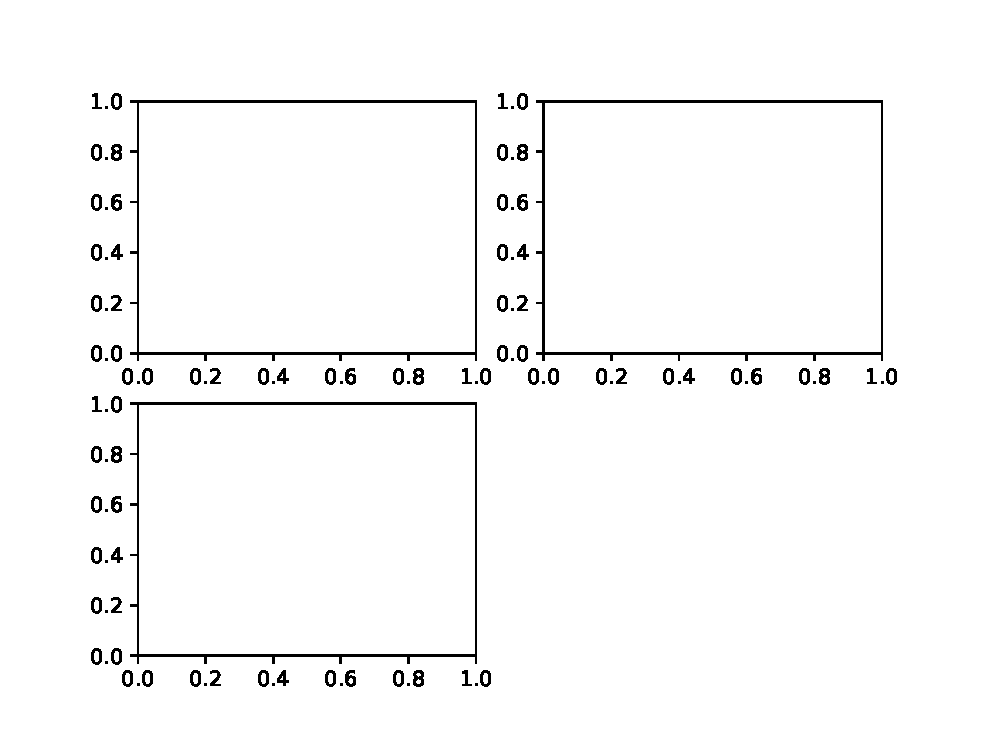
\includegraphics[width=10.0cm]{code/fig1.eps}
\endframed
\end{center}
\end{figure}
%\begin{lstlisting}
%\end{lstlisting}
\end{cod}
\vspace{-20pt}

\subsection{2次元の散布図}

2次元の散布図は,\texttt{[axes].scatter()}で描画することができる.散布図の場合は一つ一つの点がどれくらいの数値なのかがわかりにくいので,\texttt{[axes].grid()}でグリッド補助線を追加する.また,各点についてどっちが$x$でどっちが$y$かわからないので横軸と縦軸に\texttt{[axes].set\_xlabel([str])},\texttt{[axes].set\_ylabel([str])}でラベルをつける.
\begin{gram} 
\begin{itemize}
\item \texttt{[axes].scatter(x,y)}: 2次元データ$(\bm{x},\bm{y})$の散布図を描画する.ここで,$\bm{x},\bm{y}$は\texttt{ndarray}オブジェクトであり,左のデータが横軸,右のデータが縦軸である.
\item \texttt{[axes].grid()}: \texttt{axes}オブジェクトにグリッド補助線を追加する.
\item \texttt{[axes].set\_xlabel([str])}: \texttt{axes}オブジェクトの横軸にラベルをつける.
\item \texttt{[axes].set\_ylabel([str])}: \texttt{axes}オブジェクトの縦軸にラベルをつける.
\end{itemize}
\end{gram}


\begin{rem}
基本的にmatplotlibに渡すデータは,\texttt{ndarray}オブジェクトであることが必要なので,以降はその前提とする.
\end{rem}

\begin{cod}[\texttt{fig2.py}] 
\lstinputlisting[backgroundcolor={\color[gray]{.95}}]{code/fig2.py}
\vspace{-19pt}
\begin{figure}[H]
\begin{center}
\framed
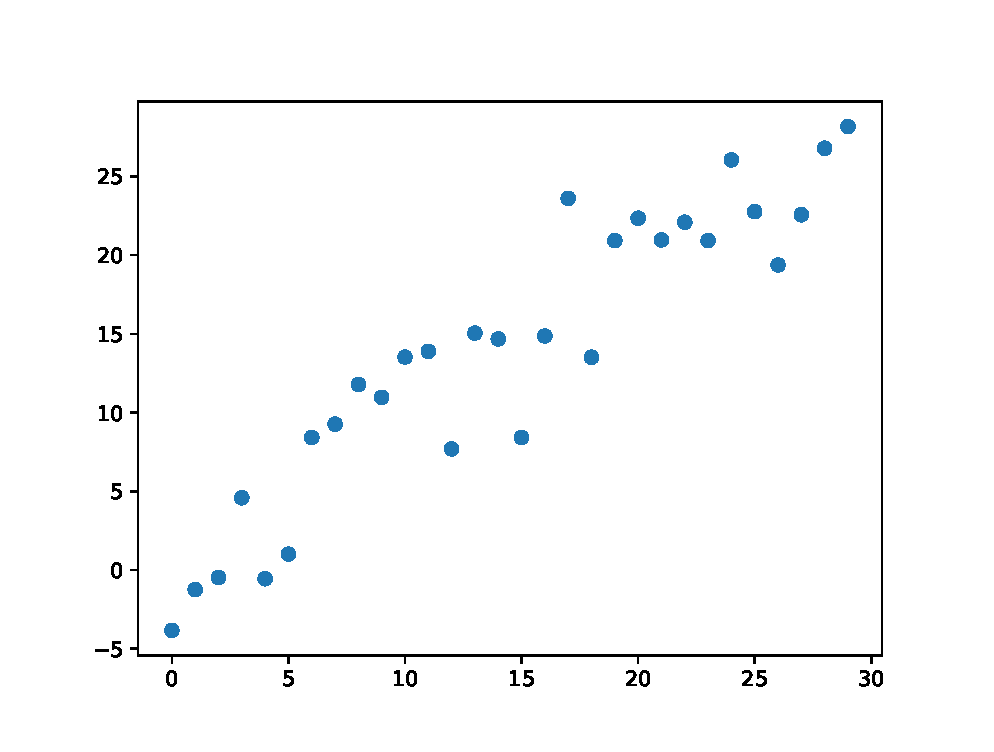
\includegraphics[width=8.0cm]{code/fig2.eps}
\endframed
\end{center}
\end{figure}
%\begin{lstlisting}
%\end{lstlisting}
\end{cod}
\vspace{-20pt}